\documentclass{article}

\usepackage{bookmark}
\usepackage{tocloft} % Add this package for table of contents


% Language setting
\usepackage[T1]{fontenc}
\usepackage[french]{babel}

% Set page size and margins
\usepackage[letterpaper,top=2cm,bottom=2cm,left=3cm,right=3cm,marginparwidth=1.75cm]{geometry}
\usepackage{float}
% Useful packages
\usepackage{amsmath}
\usepackage{graphicx}



\title{Rapport d'Analyse SonarQube}
\author{Adil ABBADI \and Abdelhak MEKAOUI}
\date{10 Octobre 2024}
\begin{document}
\maketitle

\newpage

\begin{abstract}
    Ce rapport présente les résultats de l'analyse de code effectuée avec SonarQube sur un projet Spring Boot pour la gestion des formations e-learning.
    \end{abstract}


\tableofcontents
\newpage


\section{Introduction}

Ce document décrit l'utilisation de SonarQube pour analyser un projet Spring Boot dédié à la gestion des formations e-learning. SonarQube est un outil puissant pour l'inspection continue de la qualité du code, permettant de détecter les bugs, les vulnérabilités et les mauvaises pratiques.

\section{Contexte et Objectifs}

Dans le cadre de ce module, on est chargé d’évaluer et d’améliorer la qualité d’un projet Spring Boot developpé lors d’un précédent cycle. Le projet comporte une analyse approfondie du code source à l'aide de SonarQube, des tests logiciels (boîte blanche, boîte noire, et performance), ainsi que l’intégration d’outils et de méthodologies modernes de qualité logicielle. L’objectif est de détecter, analyser, et corriger les erreurs, tout en mettant en place des solutions d’amélioration continue basées sur les principes DevOps.

\section{Résultats Attendus}

\subsection{Contexte du projet}

\begin{enumerate}
    \item Présentation du projet logiciel. \\
    Le projet consiste en une application web de gestion des formations e-learning, permettant aux utilisateurs de s’inscrire, de suivre des cours, et de passer des évaluations en ligne.
    \begin{figure}[H]
    \centering
    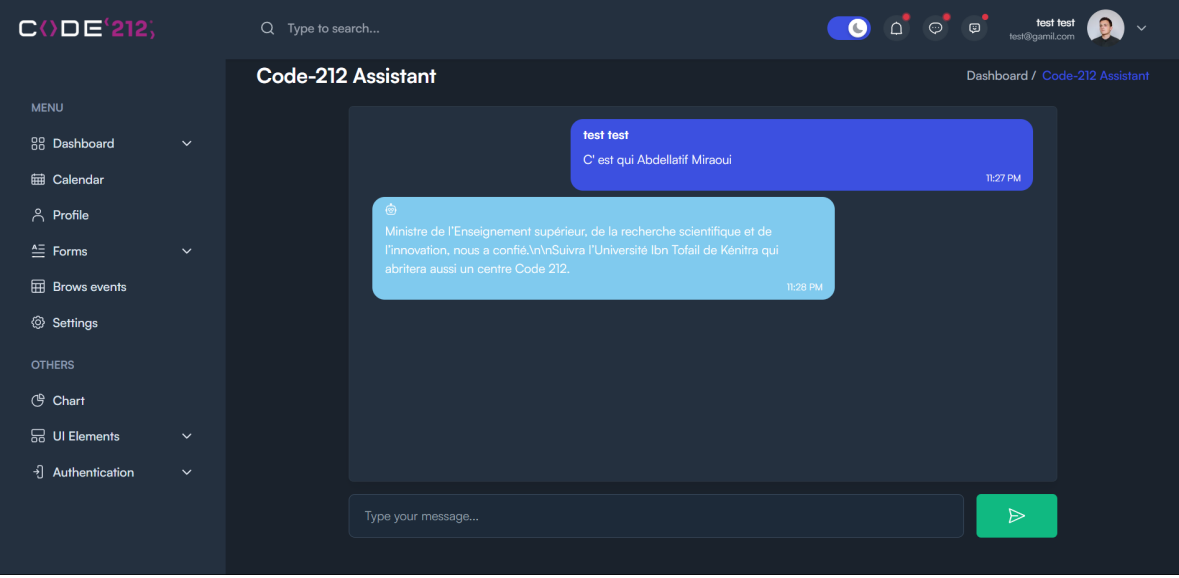
\includegraphics[width=0.8\linewidth]{assets/Screenshot 2024-12-15 192310.png}
    \caption{\label{fig:frog1}Interface utilisateur du logiciel .}
    \end{figure}

    \item Les erreurs rencontrées. \\
    Durant le développement et l'utilisation de l'application, plusieurs erreurs ont été identifiées, notamment des bugs fonctionnels, des problèmes de performance, et des vulnérabilités de sécurité.

    \item Les méthodes employées pour détecter les erreurs. \\
    Pour détecter les erreurs, diverses méthodes ont été utilisées, telles que les tests manuels, les tests automatisés, les revues de code, et l'analyse statique du code avec des outils comme SonarQube.
    \begin{figure}[H]
      \centering
      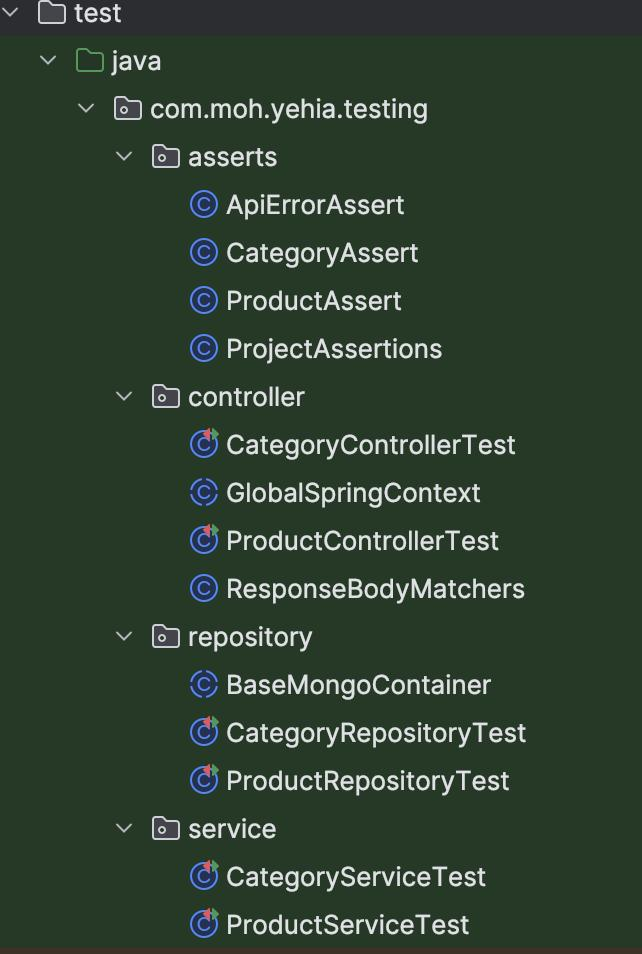
\includegraphics[width=0.5\linewidth]{assets/IMG-20241214-WA0001.jpg}
      \caption{\label{fig:froga1}Presentation du projet.}
      \end{figure}
      Github repo: \url{https://github.com/Abdelhak-mekaoui/spring-boot-ci-cd}

\end{enumerate}

\subsection{Analyse de la qualité avec SonarQube}
\begin{figure}[H]
  \centering
  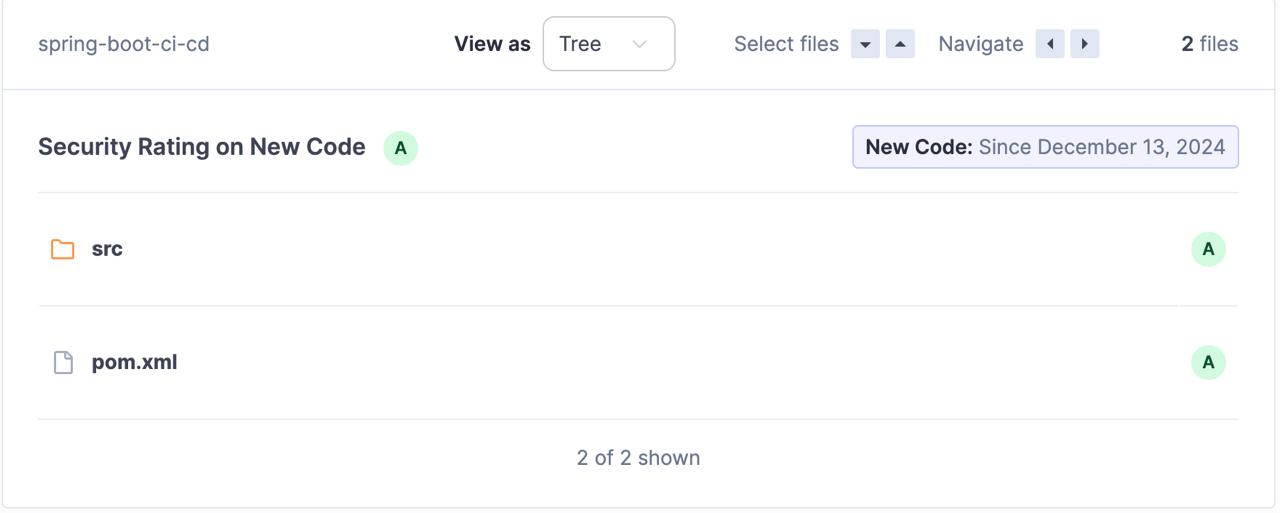
\includegraphics[width=0.9\linewidth]{assets/IMG-20241215-WA0008.jpg}
  \caption{\label{fig:frog2} Impression de l'ecran .}
  \end{figure}
\begin{enumerate}
    \item Installer ou configurer un serveur SonarQube localement .
 
    \item Importer le code source du projet précédent dans SonarQube .
 
    
    \item Examiner les métriques générées par SonarQube.
   
    \item Identifier les points faibles et proposer des améliorations.
   
\end{enumerate}

\subsection{Tests Boîte Blanche}

\begin{enumerate}
    \item Les tests unitaires.
      \begin{figure}[H]
    \centering
    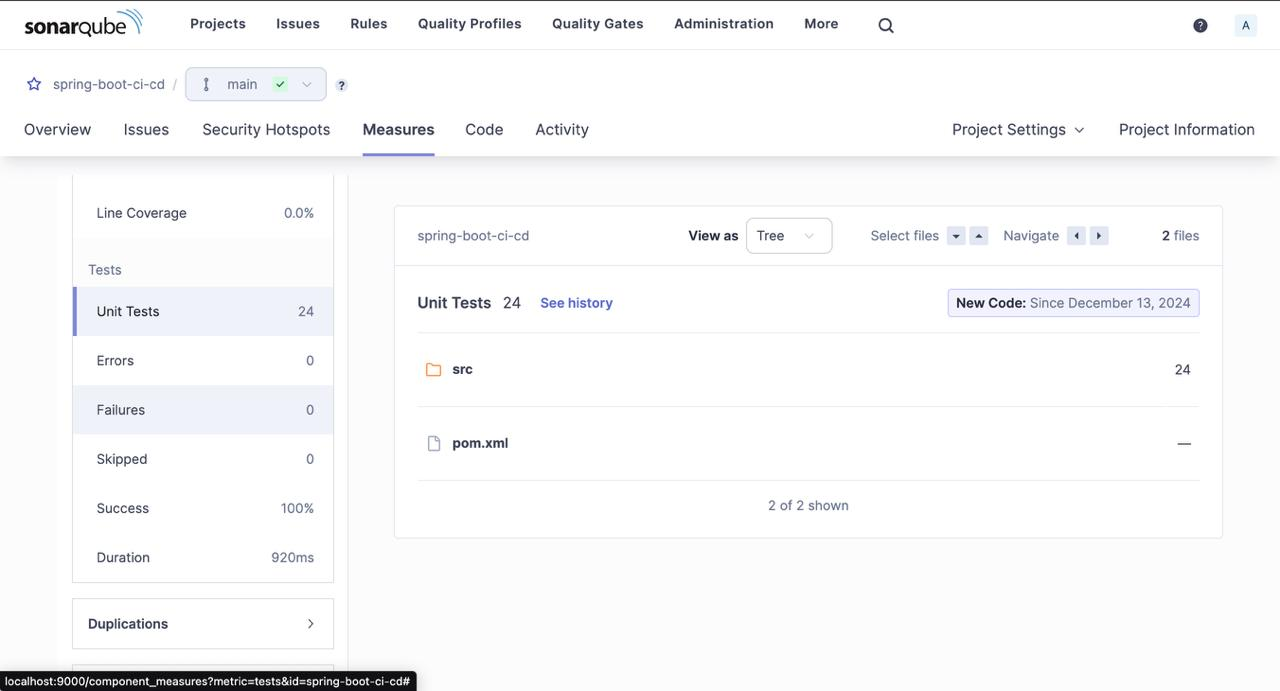
\includegraphics[width=1\linewidth]{assets/IMG-20241215-WA0005.jpg}
    \caption{\label{fig:frog6} Impression de l'ecran .}
    \end{figure}

    \item Réévaluer la couverture de code avec SonarQube après chaque itération des tests.
      \begin{figure}[H]
    \centering
    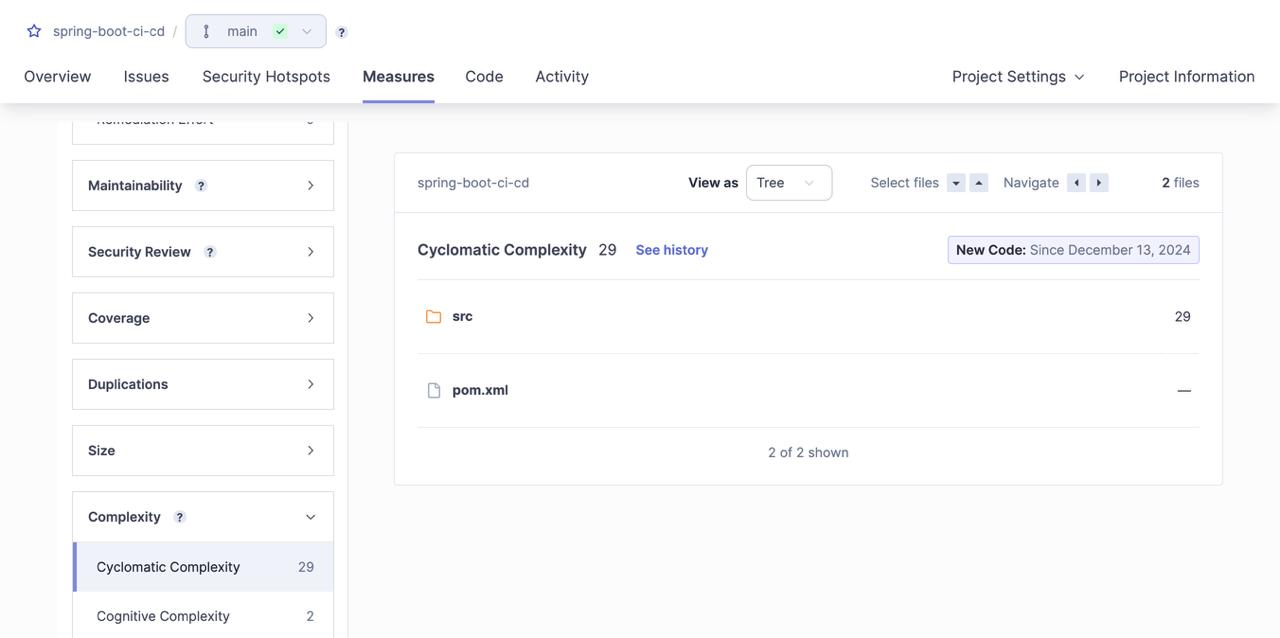
\includegraphics[width=1\linewidth]{assets/IMG-20241215-WA0007.jpg}
    \caption{\label{fig:frog7} Impression de l'ecran .}
    \end{figure}




    \item Documenter l’efficacité des tests en mettant en avant les erreurs détectées et corrigées.
      \begin{figure}[H]
    \centering
    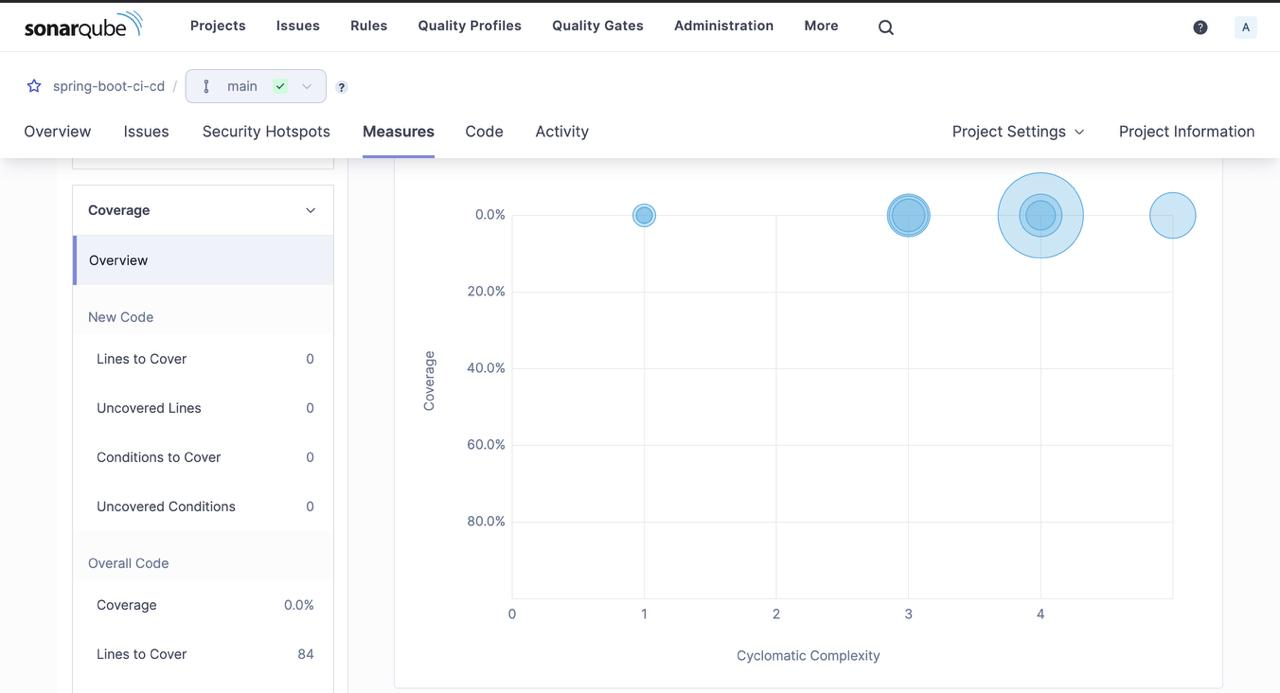
\includegraphics[width=1\linewidth]{assets/IMG-20241215-WA0009.jpg}
    \caption{\label{fig:frog8} Impression de l'ecran .}
    \end{figure}

\end{enumerate}

\subsection{Tests Boîte Noire}

\begin{enumerate}
    \item Utilisation de selenium pour simuler utilisation de application.
      \begin{figure}[H]
    \centering
    
\includegraphics[width=0.5\linewidth]{assets/selenium.png}
    \caption{\label{fig:frog9} Impression de l'ecran .}
    \end{figure}
    \newpage
    \item Tester les principales fonctionnalités de l’application en suivant différents cas d’utilisation.
  
\begin{verbatim}
  import org.openqa.selenium.By;
  import org.openqa.selenium.WebDriver;
  import org.openqa.selenium.WebElement;
  import org.openqa.selenium.chrome.ChromeDriver;
  
  public class DarkModeTest {
      public static void main(String[] args) {
          // Set the path to the chromedriver executable
          System.setProperty("webdriver.chrome.driver", "/path/to/chromedriver");
  
          // Initialize a new ChromeDriver instance
          WebDriver driver = new ChromeDriver();
  
          try {
              // Navigate to the web application
              driver.get("http://your-web-app-url.com");
  
              // Locate and click the button or switch to enable dark mode
              WebElement darkModeButton = driver.findElement(By.id("dark-mode-toggle"));
              darkModeButton.click();
  
              // Verify that dark mode is enabled
              WebElement body = driver.findElement(By.tagName("body"));
              String bodyClass = body.getAttribute("class");
              if (bodyClass.contains("dark-mode")) {
                  System.out.println("Dark mode is enabled.");
              } else {
                  System.out.println("Dark mode is not enabled.");
              }
          } finally {
              // Close the browser
              driver.quit();
          }
      }
  }
  \end{verbatim}
\end{enumerate}

\subsection{Tests de Performance}

\begin{enumerate}
    \item Test de performance tel que JMeter.
      \begin{figure}[H]
    \centering
    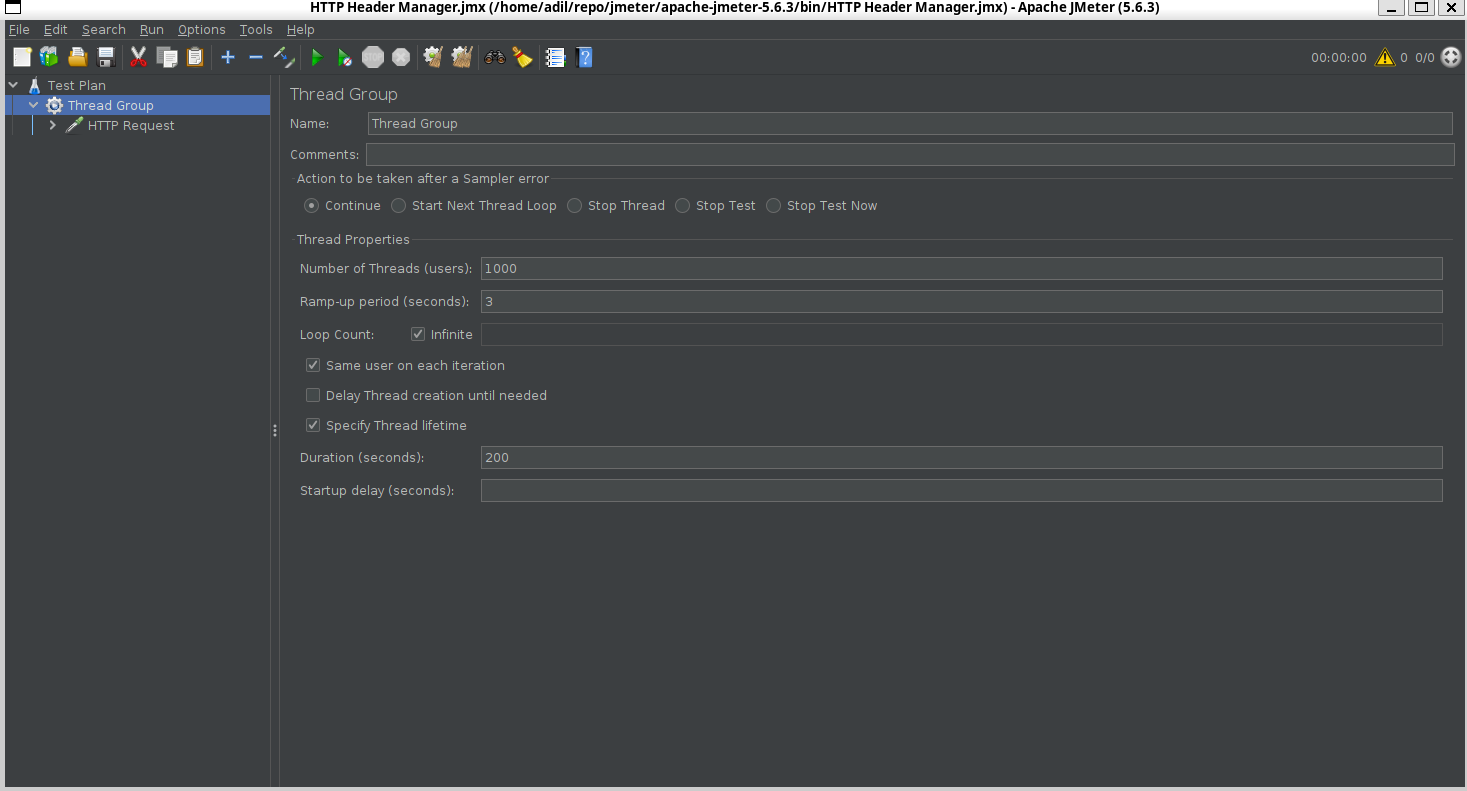
\includegraphics[width=1\linewidth]{assets/Screenshot 2024-12-15 193747.png}
    \caption{\label{fig:frog11} Impression de l'ecran .}
    \end{figure}
    \item Test de stress en simulant 500 utilisateurs.
     
    \item Test de charge, en doublant puis en triplant le nombre maximal d’utilisateurs.
      \begin{figure}[H]
    \centering
    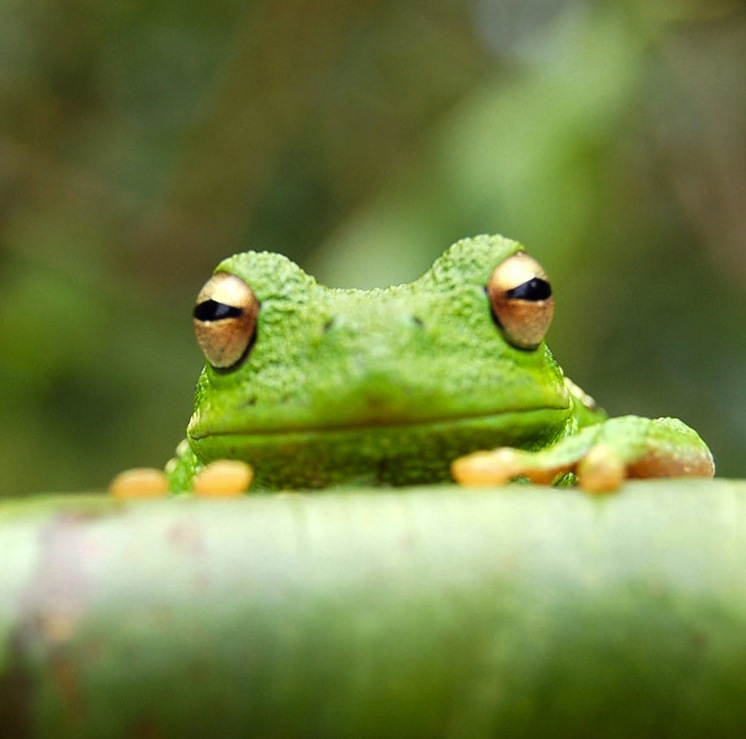
\includegraphics[width=0.5\linewidth]{assets/frog.jpg}
    \caption{\label{fig:frog13} Impression de l'ecran .}
    \end{figure}
\end{enumerate}

\subsection{Intégration DevOps et Automatisation des Tests}

\begin{enumerate}
    \item CI/CD en utilisant Jenkins .
      \begin{figure}[H]
    \centering
    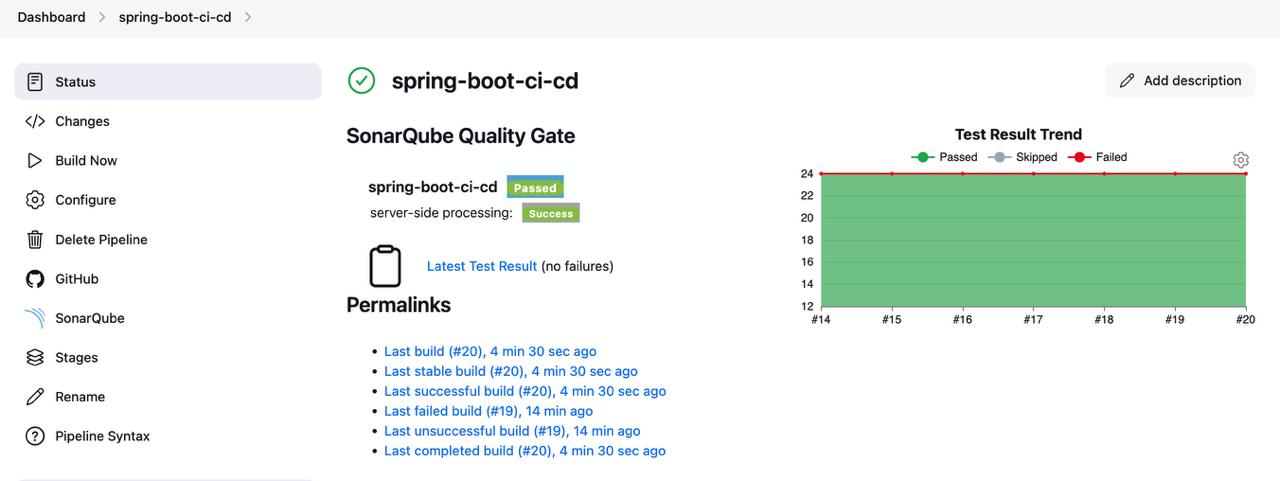
\includegraphics[width=1\linewidth]{assets/IMG-20241214-WA0006.jpg}
    \caption{\label{fig:frog14} Impression de l'ecran .}
    \end{figure}
    \item Configurer des alertes pour signaler les échecs de tests.
      \begin{figure}[H]
    \centering
    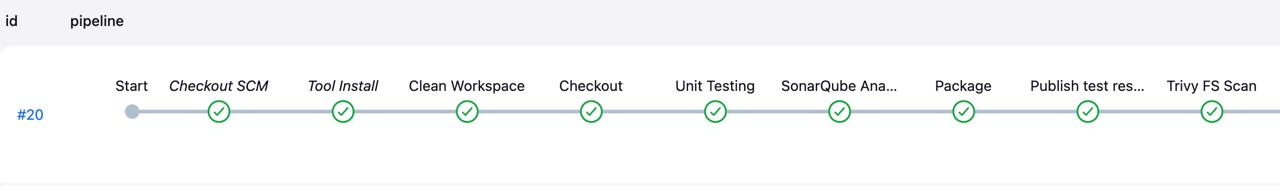
\includegraphics[width=1\linewidth]{assets/IMG-20241214-WA0002.jpg}
    \caption{\label{fig:frog15} Impression de l'ecran .}
    \end{figure}
    \item Automatiser le déploiement continu des versions en utilisant webhook.
      \begin{figure}[H]
    \centering
    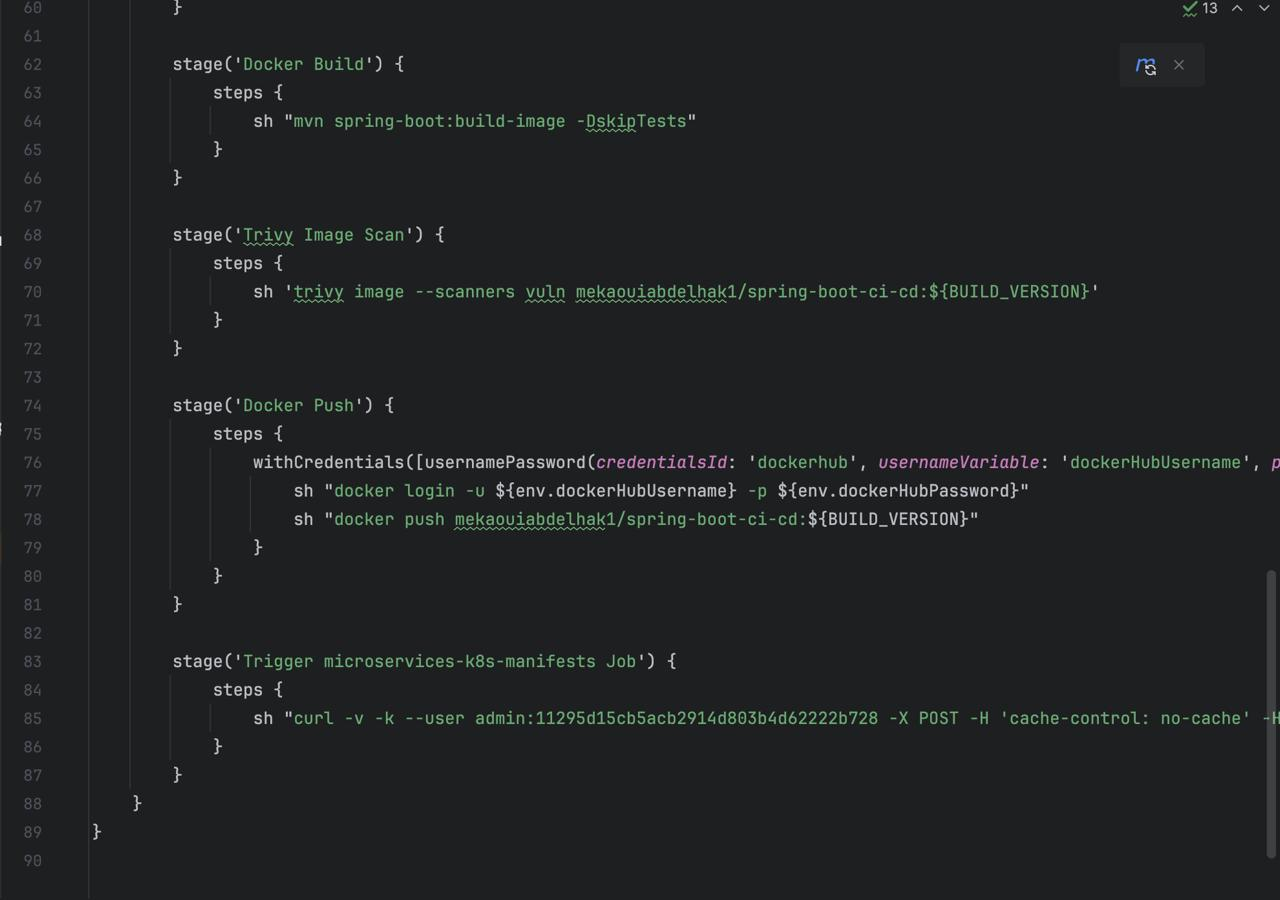
\includegraphics[width=1\linewidth]{assets/IMG-20241214-WA0009.jpg}
    \caption{\label{fig:frog16} Impression de l'ecran .}
    \end{figure}
\end{enumerate}


\section{Résultats de l'Analyse}

Les résultats de l'analyse SonarQube sont présentés ci-dessous. Ils incluent des métriques sur la qualité du code, les bugs détectés, les vulnérabilités et les duplications de code.


\subsection{Qualité du Code}

  \begin{figure}[H]
    \centering
    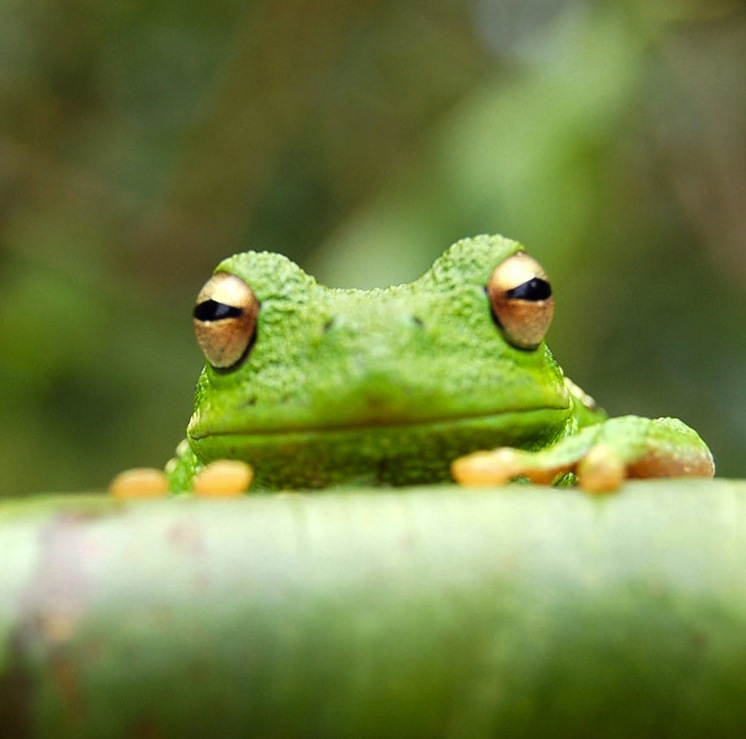
\includegraphics[width=0.5\linewidth]{assets/frog.jpg}
    \caption{\label{fig:frog17} Impression de l'ecran .}
    \end{figure}
\subsection{Bugs et Vulnérabilités}

  \begin{figure}[H]
    \centering
    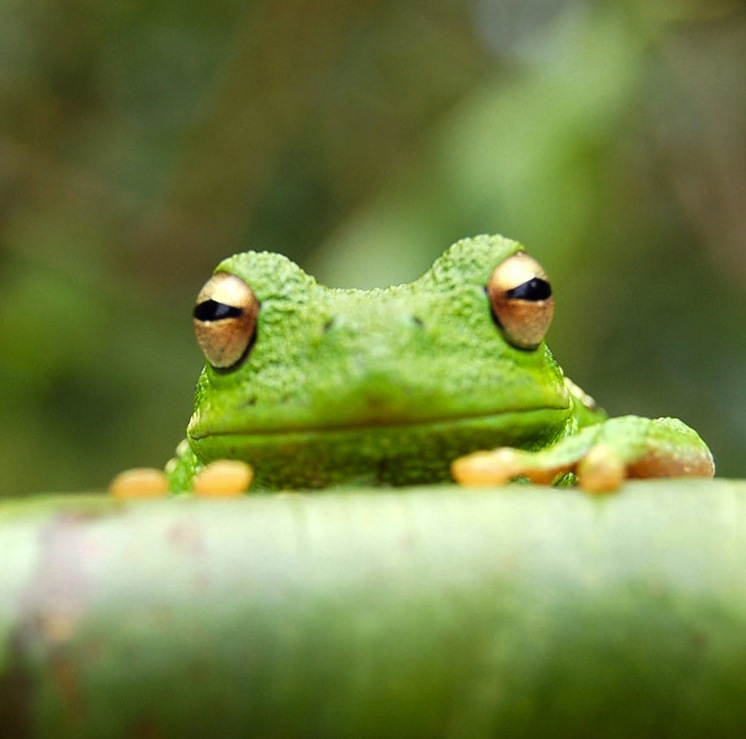
\includegraphics[width=0.5\linewidth]{assets/frog.jpg}
    \caption{\label{fig:frog18} Impression de l'ecran .}
    \end{figure}
\subsection{Duplications de Code}

  \begin{figure}[H]
    \centering
    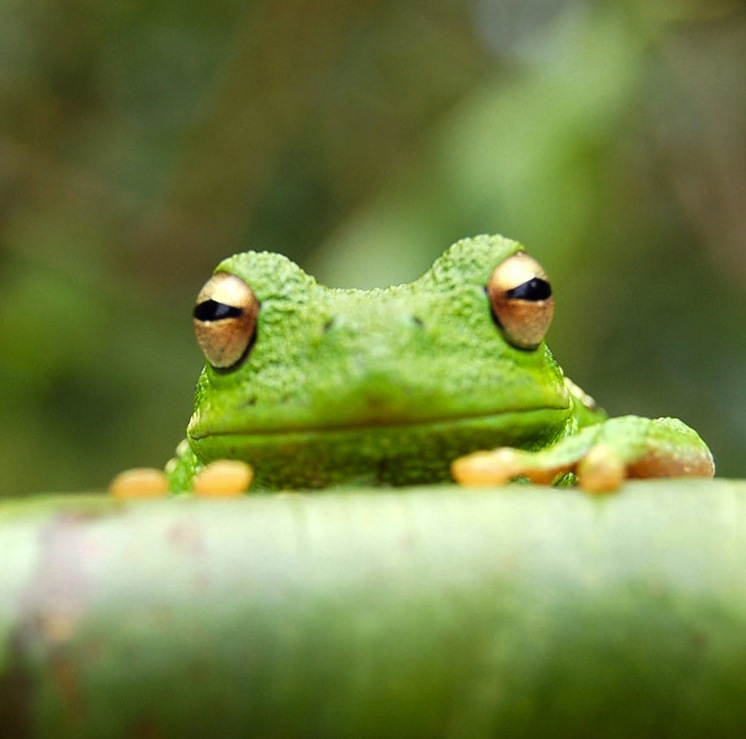
\includegraphics[width=0.5\linewidth]{assets/frog.jpg}
    \caption{\label{fig:frog19} Impression de l'ecran .}
    \end{figure}
\section{Conclusion}

En conclusion, l'utilisation de SonarQube pour analyser le projet Spring Boot de gestion des formations e-learning a permis d'identifier plusieurs aspects à améliorer en termes de qualité du code, de sécurité et de maintenabilité. Les résultats obtenus fournissent une base solide pour des améliorations futures.


% \cite{some_reference}




\end{document}